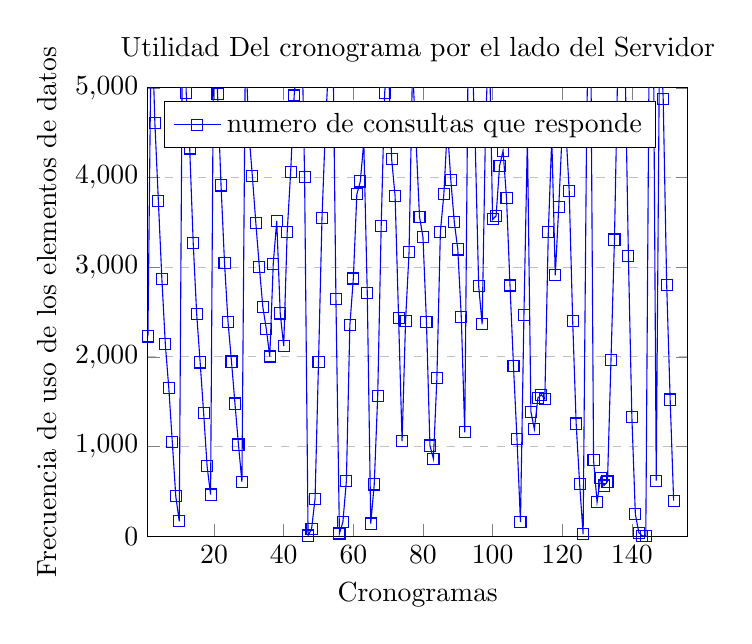
\begin{tikzpicture}
\begin{axis}[
    title={Utilidad Del cronograma por el lado del Servidor},
    xlabel={Cronogramas},
    ylabel={Frecuencia de uso de los elementos de datos},
    xmin=1, xmax=156,
    ymin=0, ymax=5000,
    xtick={},
    ytick={},
    legend pos=north west,
    ymajorgrids=true,
    grid style=dashed,
]

\addplot[
    color=blue,
    mark=square,
    ]
    coordinates {
%UTILIDAD TOTAL
(1,2228)
(2,5910)
(3,4605)
(4,3737)
(5,2872)
(6,2140)
(7,1649)
(8,1051)
(9,445)
(10,165)
(11,6198)
(12,4939)
(13,4324)
(14,3274)
(15,2481)
(16,1938)
(17,1374)
(18,779)
(19,464)
(20,6409)
(21,4934)
(22,3912)
(23,3048)
(24,2393)
(25,1948)
(26,1479)
(27,1022)
(28,605)
(29,5490)
(30,4501)
(31,4013)
(32,3491)
(33,3002)
(34,2558)
(35,2310)
(36,2004)
(37,3040)
(38,3516)
(39,2484)
(40,2120)
(41,3389)
(42,4066)
(43,4915)
(44,5332)
(45,6054)
(46,4010)
(47,7)
(48,79)
(49,416)
(50,1944)
(51,3551)
(52,4578)
(53,5361)
(54,6029)
(55,2641)
(56,30)
(57,157)
(58,617)
(59,2352)
(60,2874)
(61,3812)
(62,3956)
(63,4396)
(64,2709)
(65,141)
(66,577)
(67,1567)
(68,3461)
(69,4946)
(70,5366)
(71,4206)
(72,3790)
(73,2431)
(74,1058)
(75,2402)
(76,3165)
(77,5241)
(78,4421)
(79,3564)
(80,3333)
(81,2389)
(82,1011)
(83,865)
(84,1765)
(85,3395)
(86,3816)
(87,4567)
(88,3969)
(89,3503)
(90,3198)
(91,2449)
(92,1158)
(93,5524)
(94,5507)
(95,4397)
(96,2791)
(97,2363)
(98,4627)
(99,5641)
(100,3533)
(101,3572)
(102,4129)
(103,4301)
(104,3770)
(105,2796)
(106,1896)
(107,1088)
(108,156)
(109,2471)
(110,4450)
(111,1387)
(112,1194)
(113,1541)
(114,1578)
(115,1529)
(116,3390)
(117,4438)
(118,2909)
(119,3673)
(120,4523)
(121,4563)
(122,3849)
(123,2402)
(124,1256)
(125,582)
(126,21)
(127,4530)
(128,6764)
(129,846)
(130,381)
(131,652)
(132,565)
(133,609)
(134,1963)
(135,3308)
(136,5348)
(137,6937)
(138,5415)
(139,3128)
(140,1332)
(141,245)
(142,40)
(143,4)
(144,0)
(145,5640)
(146,6863)
(147,619)
(148,5831)
(149,4875)
(150,2804)
(151,1524)
(152,396)
    };
    \legend{numero de consultas que responde}

\end{axis}
\end{tikzpicture}

